\newpage
\section{Diseño del Sistema}

En este capítulo se describe la solución técnica adoptada para satisfacer los requisitos expuestos en la fase de análisis. Se detalla la arquitectura del sistema desde dos perspectivas complementarias: la arquitectura física (despliegue) y la arquitectura lógica (componentes), justificando las decisiones tecnológicas adoptadas para el ecosistema de MoodNest.

\subsection{Diseño de la Arquitectura Física y Despliegue}

En este apartado se detalla la infraestructura física y el entorno de ejecución sobre el cual se asienta MoodNest. Para garantizar la portabilidad, la escalabilidad y la facilidad de despliegue, se ha adoptado una arquitectura basada en contenedores utilizando la tecnología Docker.

Como se observa en el Diagrama de Despliegue de la Figura \ref{fig:diagrama_despliegue}, el sistema se distribuye en dos nodos principales que interactúan a través de redes estándar de comunicación:

\begin{itemize}
    \item \textbf{Nodo Cliente (Dispositivo del Usuario):} Representa el hardware físico desde el cual el usuario accede a la plataforma (PC, tablet o smartphone). El software no requiere instalación local, ya que el artefacto \textit{MoodNest SPA} (desarrollado en React.js) se ejecuta directamente dentro de un Navegador Web. Al ser una \textit{Single Page Application}, la lógica de presentación y navegación opera localmente en el cliente tras la carga inicial.
    
    \item \textbf{Nodo Servidor (Servidor Anfitrión / Host):} Representa la máquina física o virtual que aloja la lógica central y los datos de la aplicación. Este equipo ejecuta un \textit{Docker Engine} encargado de orquestar tres contenedores independientes y aislados:
    \begin{enumerate}
        \item \textbf{Contenedor Frontend:} Actúa como servidor de archivos estáticos que entrega la SPA al navegador web cuando se realiza la primera conexión.
        \item \textbf{Contenedor Backend:} Contiene un entorno de ejecución Java que corre la aplicación Spring Boot junto a su servidor Tomcat embebido, exponiendo los \textit{endpoints} de la API REST.
        \item \textbf{Contenedor de Base de Datos:} Provee el servicio de persistencia mediante el motor NoSQL MongoDB, encapsulado y protegido de forma que solo sea accesible mediante la red interna de Docker.
    \end{enumerate}
\end{itemize}

La integridad del sistema se apoya en flujos de comunicación diferenciados: los recursos estáticos y las peticiones a la API REST viajan a través del protocolo \textbf{HTTPS} (intercambiando información en formato JSON), mientras que la comunicación interna de alto rendimiento entre la API y la base de datos se realiza mediante \textbf{TCP/IP} utilizando el \textit{Mongo Java Driver}.

\begin{figure}[h!]
    \centering
    % Ajusta el tamaño de la imagen según necesites
    \includegraphics[width=0.95\textwidth]{Imagenes/diagrama_despliegue.pdf}
    \caption{Diagrama de Despliegue físico de la plataforma MoodNest}
    \label{fig:diagrama_despliegue}
\end{figure}


\subsection{Arquitectura Lógica del Sistema}

Una vez definida la infraestructura física y el entorno de ejecución, es fundamental detallar la organización interna del software de MoodNest. El diseño de la arquitectura lógica no es una mera distribución de archivos, sino la materialización de los principios de ingeniería de software de \textbf{alta cohesión} y \textbf{bajo acoplamiento}. 

El objetivo primordial de esta estructura es garantizar que el sistema sea mantenible a largo plazo y fácilmente escalable. Para ello, se ha optado por una arquitectura desacoplada que separa la lógica de presentación de la lógica de negocio y la persistencia de datos. Esta organización permite que los cambios en una capa (por ejemplo, una actualización en la interfaz visual) tengan un impacto nulo o mínimo en las demás capas (como la base de datos). Para representar esta estructura, se han elaborado un Diagrama de Componentes y un Diagrama de Paquetes siguiendo el estándar UML.

\subsubsection{Diseño de Componentes}

El Diagrama de Componentes (Figura \ref{fig:diagrama_componentes}) ofrece una visión de alto nivel de los módulos funcionales que componen MoodNest y, lo más importante, de cómo estos interactúan a través de interfaces explícitas. 



En esta vista, el sistema se divide en tres estratos principales, cada uno con una responsabilidad única y bien definida:

\begin{itemize}
    \item \textbf{Capa de Presentación (Frontend):} Se materializa en el componente \texttt{MoodNest SPA}. Este módulo es el encargado de toda la interacción directa con el usuario, incluyendo el renderizado de los elementos visuales de la interfaz y la gestión del estado local en el navegador. Es un componente "delgado" en términos de reglas de negocio; su función no es procesar datos, sino solicitarlos y presentarlos. Para ello, actúa como un consumidor que se conecta a los servicios del backend mediante interfaces requeridas o ''enchufes''.
    
    \item \textbf{Capa de Lógica de Negocio (Backend):} Es el núcleo del sistema, implementado sobre el framework Spring Boot. Para evitar un código monolítico y difícil de gestionar, esta capa se ha modularizado en "Gestores" independientes que encapsulan dominios de información específicos:
    \begin{itemize}
        \item \textbf{UsuariosMgr}: Centraliza la seguridad y gestión de identidad, resolviendo las operaciones críticas de registro, autenticación mediante JWT y mantenimiento del perfil de usuario.
        \item \textbf{RegistrosDiariosMgr}: Gestiona la lógica principal de la aplicación, controlando el ciclo de vida completo (creación, lectura, actualización y borrado) de las entradas de estado de ánimo diarias.
        \item \textbf{EtiquetasMgr}: Administra el catálogo de factores contextuales (actividades, personas, eventos) que el usuario puede asociar a sus registros, permitiendo una personalización total del sistema.
        \item \textbf{EstadísticasMgr}: Es el componente analítico encargado de procesar los datos en bruto para generar información de valor, como el cálculo de rachas de uso y la detección de patrones de impacto emocional entre etiquetas y humor.
    \end{itemize}

    \item \textbf{Capa de Acceso a Datos:} Representada por el componente \texttt{Base de Datos MongoDB}. Siguiendo el principio de inversión de dependencias, los gestores del backend no conocen los detalles técnicos de cómo se guardan los datos. Simplemente requieren una interfaz común de acceso (\texttt{IDataAccess}), la cual es proporcionada por este componente de persistencia. Esto permite que MoodNest sea tecnológicamente agnóstico: si en el futuro se decidiera cambiar MongoDB por otra tecnología, la lógica de negocio permanecería intacta.
\end{itemize}

\begin{figure}[H]
    \centering
    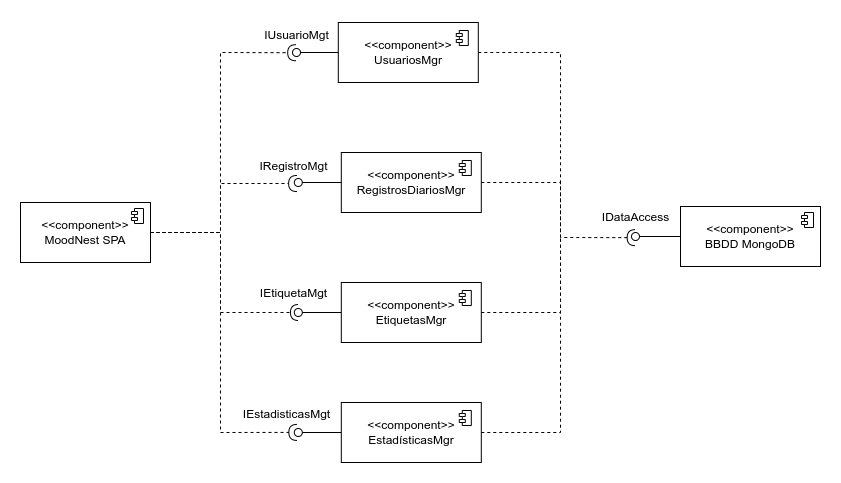
\includegraphics[width=0.9\textwidth]{Imagenes/diagrama_componentes.png}
    \caption{Diagrama de Componentes de la Arquitectura de MoodNest.}
    \label{fig:diagrama_componentes}
\end{figure}

\subsubsection{Organización del Código (Diagrama de Paquetes)}

La arquitectura lógica no solo se define por sus componentes funcionales, sino también por cómo se organiza físicamente el código fuente para garantizar la escalabilidad y el trabajo colaborativo. Para representar esta jerarquía, se ha elaborado un Diagrama de Paquetes UML (Figura \ref{fig:diagrama_paquetes}), que actúa como un mapa del proyecto, agrupando las clases y módulos según su responsabilidad técnica.

La elección de esta estructura no es arbitraria; se basa en el principio de separación de responsabilidades (\textit{Separation of Concerns}). Al dividir el proyecto en paquetes claramente delimitados, se consigue que un cambio en la lógica de acceso a datos no afecte a la interfaz de usuario, y que la lógica de negocio permanezca aislada de las peticiones HTTP.

\paragraph{Estructura del Backend (Spring Boot)}

En el servidor, se ha adoptado una \textbf{Arquitectura por Capas} (\textit{Layered Architecture}), que es el estándar en entornos empresariales con Spring Boot. Esta organización permite que el flujo de datos sea unidireccional y predecible:

\begin{itemize}
    \item \textbf{Paquete \texttt{controllers}}: Actúa como la frontera del sistema. Contiene las clases que interceptan las peticiones entrantes del cliente, validan los parámetros básicos y mapean las URLs de la API REST. Su única responsabilidad es recibir la solicitud y entregar la respuesta, delegando cualquier cálculo al siguiente nivel.
    \item \textbf{Paquete \texttt{services}}: Es el "cerebro" de la aplicación. Aquí se implementa la lógica de negocio pura, como el cálculo de rachas de días consecutivos o el análisis de impacto de las etiquetas. Al estar aislada en servicios, esta lógica puede ser reutilizada o testeada de forma independiente.
    \item \textbf{Paquete \texttt{repositories}}: Funciona como una capa de abstracción sobre MongoDB. Utiliza las interfaces de Spring Data para realizar operaciones de persistencia sin necesidad de escribir consultas manuales complejas, facilitando el mantenimiento si la tecnología de base de datos cambiara en el futuro.
    \item \textbf{Paquete \texttt{models} y \texttt{dto}}: Se ha realizado una distinción crítica entre las entidades de base de datos (\texttt{models}), que reflejan la estructura de las colecciones de MongoDB, y los Objetos de Transferencia de Datos (\texttt{dto}). Estos últimos permiten enviar al frontend únicamente la información necesaria, protegiendo datos sensibles como las contraseñas cifradas.
    \item \textbf{Paquete \texttt{security}}: Contiene la configuración de Spring Security y la lógica necesaria para interceptar y validar los tokens JWT. Es el guardián que asegura que solo los usuarios autenticados accedan a sus propios datos emocionales.
\end{itemize}



\paragraph{Estructura del Frontend (React)}

En el lado del cliente, la organización se basa en un paradigma de \textbf{Arquitectura Basada en Componentes}. El objetivo es tratar la interfaz de usuario como un conjunto de piezas de Lego reutilizables, lo que agiliza el desarrollo y garantiza la coherencia visual:

\begin{itemize}
    \item \textbf{Paquete \texttt{pages}}: Representa las vistas de alto nivel o pantallas completas a las que el usuario puede navegar (como el Panel Principal o el Calendario). Su función es orquestar los componentes más pequeños para darles sentido dentro de una ruta específica.
    \item \textbf{Paquete \texttt{components}}: Almacena los elementos visuales atómicos y reutilizables, como botones, tarjetas de registro o las visualizaciones de Chart.js. Esta separación permite modificar el diseño de un botón en un solo archivo y que el cambio se refleje en toda la aplicación.
    \item \textbf{Paquete \texttt{services}}: Encapsula toda la comunicación con el exterior. En lugar de realizar llamadas a la API directamente desde los componentes visuales, se centralizan aquí mediante librerías como Axios. Esto desacopla la interfaz de la infraestructura de red.
    \item \textbf{Paquete \texttt{context} y \texttt{hooks}}: Estos paquetes gestionan el estado global y la lógica compartida. El \texttt{context} permite que datos como la sesión del usuario o el tema visual estén disponibles en cualquier parte de la aplicación sin necesidad de pasarlos manualmente entre componentes, mientras que los \texttt{hooks} permiten reciclar lógica compleja de forma elegante.
\end{itemize}

Esta organización modular permite que MoodNest sea un sistema robusto donde cada archivo tiene un propósito único y una ubicación lógica, minimizando el riesgo de errores durante la fase de implementación y facilitando la incorporación de futuras funcionalidades.

\begin{figure}[H]
    \centering
    \includegraphics[width=0.9\textwidth]{Imagenes/diagrama_paquetes.pdf}
    \caption{Organización de paquetes y dependencias de MoodNest.}
    \label{fig:diagrama_paquetes}
\end{figure}

\newpage

\subsection{Diseño del Modelo de Datos}

El núcleo de MoodNest reside en la capacidad de almacenar, relacionar y analizar el historial emocional del usuario. A diferencia de los sistemas tradicionales, la naturaleza de los registros diarios es altamente dinámica: un registro puede contener múltiples etiquetas con puntuaciones específicas, anotaciones de longitud variable o carecer por completo de ellas. 

Para dar respuesta a esta flexibilidad sin comprometer el rendimiento, se ha descartado el modelo relacional tradicional (SQL) en favor de una base de datos NoSQL orientada a documentos, concretamente MongoDB. Este paradigma permite almacenar la información en formato BSON (Binary JSON), garantizando una lectura ágil y evitando las costosas operaciones de cruce de tablas JOINs que mermarían la escalabilidad del sistema \cita{}.

\subsubsection{Modelo Conceptual del Dominio}

El sistema se articula en torno a tres entidades principales: el \texttt{Usuario}, la \texttt{Etiqueta} y el \texttt{RegistroDiario}. La Figura \ref{fig:diagrama_conceptual} ilustra el modelo de dominio y la cardinalidad entre estos elementos. Un usuario actúa como entidad raíz, poseyendo una colección de etiquetas personalizadas y un historial de registros diarios.

\begin{figure}[H]
    \centering
    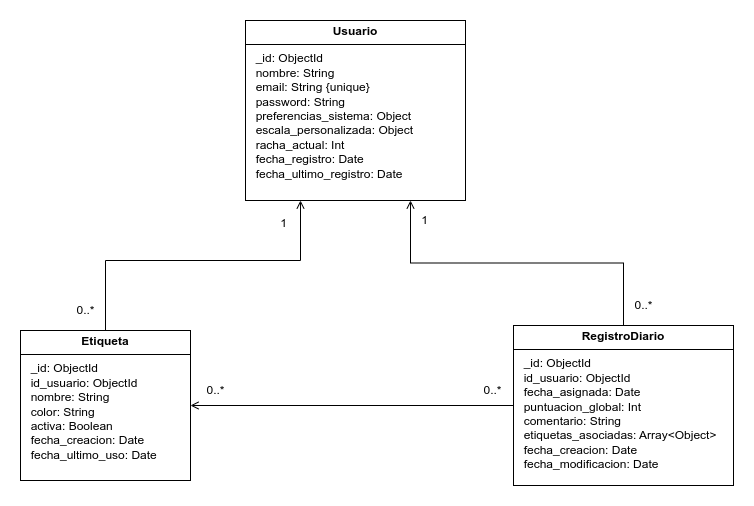
\includegraphics[width=0.8\textwidth]{Imagenes/diagrama_clases.png}
    \caption{Diagrama de Clases Conceptual del Dominio de MoodNest.}
    \label{fig:diagrama_conceptual}
\end{figure}

\subsubsection{Patrones de Diseño NoSQL y Esquemas Físicos}

En el modelado de bases de datos orientadas a documentos, es crucial definir si los datos relacionados se anidan (\textit{Embedding}) o se referencian (\textit{Referencing}) \cita{}. 

Para la relación entre los \texttt{RegistrosDiarios} y las \texttt{Etiquetas}, se ha optado por el Patrón de Referenciación. Dado que las etiquetas tienen un ciclo de vida propio (pueden ser modificadas en color o nombre, o ser desactivadas por el usuario), anidarlas dentro de cada registro diario generaría una redundancia masiva e inconsistencias en las actualizaciones históricas. Por tanto, se han diseñado tres colecciones independientes. A continuación, se detallan los esquemas físicos en formato JSON que dan cobertura a los Requisitos de Información (RI) analizados previamente.

\paragraph{Colección \texttt{usuarios}}
Almacena las credenciales de acceso, la configuración de personalización de la interfaz y escala de ánimo y las métricas de uso.

\begin{lstlisting}[style=estiloJSON]
{
  "_id": ObjectId("64b8f..."),
  "nombre": "Guillermo",
  "email": "usuario@email.com",
  "password": "$2a$10$hashed_password_string...",
  "preferencias_sistema": {
    "tema": "oscuro",
    "color_principal": "#3498db",
    "familia_iconos": "minimalista"
  },
  "escala_personalizada": {
    "1": "Terrible",
    "5": "Normal",
    "10": "Excelente"
  },
  "racha_actual": 12,
  "fecha_registro": ISODate("2026-05-01T10:00:00Z"),
  "fecha_ultimo_registro": ISODate("2026-05-09T18:30:00Z")
}
\end{lstlisting}

\paragraph{Colección \texttt{etiquetas}}
Actúa como el catálogo personalizado de factores contextuales de cada usuario. Se ha incluido un campo booleano ''activa'' para permitir un borrado lógico, garantizando que si el usuario elimina una etiqueta, esta no desaparezca de los registros históricos del pasado.

\begin{lstlisting}[style=estiloJSON]
{
  "_id": ObjectId("64c1a..."),
  "id_usuario": ObjectId("64b8f..."),
  "nombre": "Deporte",
  "color": "#2ecc71",
  "activa": true,
  "fecha_creacion": ISODate("2026-05-02T09:15:00Z"),
  "fecha_ultimo_uso": ISODate("2026-05-09T18:30:00Z")
}
\end{lstlisting}

\paragraph{Colección \texttt{registros\_diarios}}
Es la colección transaccional principal. Implementa el patrón de referenciación mediante el array \texttt{etiquetas\_asociadas}, el cual guarda únicamente el identificador de la etiqueta y la puntuación numérica opcional asignada a ese factor específico en ese día concreto.

\begin{lstlisting}[style=estiloJSON]
{
  "_id": ObjectId("64d5e..."),
  "id_usuario": ObjectId("64b8f..."),
  "fecha_asignada": ISODate("2026-05-09T00:00:00Z"),
  "puntuacion_global": 8,
  "comentario": "Hoy ha sido un dia bastante productivo.",
  "etiquetas_asociadas": [
    {
      "id_etiqueta": ObjectId("64c1a..."),
      "puntuacion": 9
    },
    {
      "id_etiqueta": ObjectId("64c2b..."),
      "puntuacion": null
    }
  ],
  "fecha_creacion": ISODate("2026-05-09T18:30:00Z"),
  "fecha_modificacion": ISODate("2026-05-09T18:30:00Z")
}
\end{lstlisting}

Con la definición de estas tres colecciones, se da por finalizado el diseño de la capa de persistencia. Esta arquitectura física basada en documentos JSON da cobertura total y estricta a los Requisitos de Información extraídos durante la fase de análisis \cita{}. La combinación de la flexibilidad inherente de MongoDB con el uso estratégico del patrón de referenciación garantiza que el modelo de datos de MoodNest sea robusto, altamente escalable y perfectamente capaz de soportar la evolución del historial emocional del usuario a lo largo de los años.


\newpage
\subsection{Diseño del Comportamiento y Seguridad}

El diseño del comportamiento de MoodNest se centra en garantizar una interacción fluida entre el cliente y el servidor, bajo un estricto marco de seguridad que cumpla con el \textbf{RNF4.2 (Protección de datos privados)} \cita{}.

A diferencia de las arquitecturas web tradicionales basadas en sesiones de servidor (\textit{Stateful}), MoodNest implementa una arquitectura \textit{Stateless} mediante el uso de "JSON Web Tokens (JWT)" \cita{}. Esta elección responde a la necesidad de optimizar la escalabilidad del sistema. El JWT consiste en un token digital firmado criptográficamente que funciona como una credencial de identidad autónoma. Al utilizar este mecanismo, el servidor no necesita reservar memoria para mantener el estado de cada usuario; en su lugar, delega en el cliente la responsabilidad de portar su propia identidad en la cabecera de cada petición. Este token viaja codificado y contiene la información mínima necesaria (el identificador del usuario y la fecha de caducidad) asegurando mediante una firma secreta en el backend que la información no ha sido manipulada por terceros. De este modo, se garantiza un acceso seguro a los datos emocionales sin comprometer el rendimiento del servidor.

Para entender mejor cómo MoodNest integra este mecanismo de seguridad, analizaremos tanto el flujo de autenticación y generación del JWT como el proceso de validación que sigue la plataforma para proteger la información del usuario en cada solicitud de acceso a datos sensibles. 

\subsubsection{Fase 1: Autenticación y Generación de Credenciales}

El proceso de seguridad comienza con la identificación del usuario. La Figura \ref{fig:gen_jwt} ilustra la dinámica de autenticación mediante un diagrama de secuencia. Por motivos de claridad técnica, este diagrama se centra en un flujo ideal de inicio de sesión, asumiendo que el flujo de control se gestiona mediante excepciones globales en caso de error en las credenciales.

\begin{figure}[H]
    \centering
    \includegraphics[width=0.9\textwidth]{Imagenes/diagrama_secuencia_generacionJWT.pdf}
    \caption{Diagrama de secuencia: Proceso de login y generación de JWT.}
    \label{fig:gen_jwt}
\end{figure}

En este flujo, una vez que el componente \texttt{UsuariosMgr} valida la coincidencia del \textit{hash} de la contraseña, el \texttt{JwtService} emite un token firmado. Este es devuelto al navegador en una respuesta \texttt{200 OK} y almacenado de forma persistente en el \texttt{localStorage} del cliente, permitiendo mantener la sesión activa tras recargas de página.

\subsubsection{Fase 2: Acceso a Recursos y Validación de Seguridad}

Cada petición dirigida a un recurso protegido, como la consulta del historial de registros emocionales, requiere la validación de la identidad. Este proceso es crítico para garantizar que ningún usuario pueda acceder a datos ajenos.

\begin{figure}[H]
    \centering
    \includegraphics[width=0.9\textwidth]{Imagenes/diagrama_secuencia_validacionJWT.pdf}
    \caption{Diagrama de secuencia: Validación de token y acceso a datos privados.}
    \label{fig:val_jwt}
\end{figure}

Como se observa en la Figura \ref{fig:val_jwt}, el servidor no confía ciegamente en el token recibido y realiza un proceso de validación en tres capas antes de conceder acceso a los datos sensibles:

\begin{itemize}
  \item \textbf{Comprobación de autenticidad:} Cuando el backend recibe el token, utiliza una clave secreta que solo el servidor conoce para recalcular la firma de los datos recibidos. Si el resultado de este cálculo coincide con la firma que acompaña al token, el servidor confirma que la identidad del usuario es auténtica y que nadie ha modificado su contenido durante el trayecto.
  \item \textbf{Verificación de caducidad:} El sistema comprueba que el token todavía se encuentra dentro de su periodo de validez. Si el tiempo ha expirado, el acceso se deniega automáticamente por seguridad.
  \item \textbf{Acceso restringido a los datos:} Una vez que el token es validado, el servidor extrae el identificador único del usuario que viaja en su interior. Este identificador es el que se utiliza obligatoriamente para filtrar las consultas a la base de datos MongoDB. De esta manera, el sistema garantiza que un usuario solo pueda visualizar o gestionar sus propios registros, bloqueando cualquier intento de acceso a información ajena.
\end{itemize}

Gracias a este mecanismo, la seguridad de MoodNest no depende de mantener una conexión constante, sino de la validez de la credencial que el usuario presenta en cada interacción.

\newpage
\subsection{Diseño de Interfaz y Guía de Estilo Visual}

El diseño de la interfaz de MoodNest se ha concebido bajo los principios de usabilidad, claridad y "cero fricción". A continuación se detallan los elementos que componen la identidad visual del sistema.

\subsubsection{Identidad de Marca y Logotipo}

Para la identidad gráfica de MoodNest se ha diseñado un isotipo que fusiona el monograma de la marca con su funcionalidad principal. El logotipo consiste en una línea continua en forma de cinta que dibuja la letra "M", finalizando en una flecha ascendente.

\begin{figure}[H]
    \centering
    
\includegraphics[width=0.4\textwidth]{Imagenes/logo_moodnest.png}
    \caption{Logotipo oficial de MoodNest: Monograma con tendencia ascendente.}
    \label{fig:logo_marca}
\end{figure}

Esta simbología representa la continuidad del registro diario y el objetivo de crecimiento personal del usuario.

\subsubsection{Paleta de Colores Corporativa}

Se ha definido una paleta de colores que induce a la calma, utilizando el azul noche para garantizar una lectura cómoda.

\begin{itemize}
    \item \colorboxsquare{MoodPrimario} \textbf{Color Primario (\texttt{\#5B61C4}):} Identidad principal y botones de acción.
    \item \colorboxsquare{MoodSecundario} \textbf{Color Secundario (\texttt{\#A9ACE0}):} Elementos de apoyo y acentos visuales.
    \item \colorboxsquare{MoodTexto} \textbf{Color de Texto (\texttt{\#1E1E2F}):} Azul noche profundo para legibilidad máxima.
    \item \colorboxsquare{white} \textbf{Fondos (\texttt{\#F8F9FA}):} Lienzo neutro para reducir la fatiga visual.
\end{itemize}

\subsubsection{Escala Semántica Emocional}

Para representar las puntuaciones del 1 al 10 de forma intuitiva, se utiliza la siguiente escala cromática:

\begin{itemize}
    \item \colorboxsquare{MoodTerrible} \textbf{1 - 2 (\texttt{\#EF4444}):} Rojo - Estado de malestar agudo.
    \item \colorboxsquare{MoodRegular} \textbf{3 - 4 (\texttt{\#F97316}):} Naranja - Tensión o incomodidad.
    \item \colorboxsquare{MoodNormal} \textbf{5 - 6 (\texttt{\#EAB308}):} Amarillo - Estado neutro.
    \item \colorboxsquare{MoodBien} \textbf{7 - 8 (\texttt{\#84CC16}):} Verde Lima - Tranquilidad y bienestar.
    \item \colorboxsquare{MoodPrimario} \textbf{9 - 10 (\texttt{\#5B61C4}):} Índigo Primario - Máximo bienestar y éxito emocional.
\end{itemize}

\subsubsection{Tipografía}

La jerarquía de textos combina elegancia y funcionalidad técnica:

\begin{itemize}
    \item \textbf{PT Serif:} Reservada para títulos y encabezados. Aporta un carácter reflexivo y humano.
    \item \textbf{Lato:} Utilizada para el contenido dinámico y formularios por su alta legibilidad.
\end{itemize}

\begin{figure}[H]
    \centering
    
\includegraphics[width=0.8\textwidth]{Imagenes/tipografia_moodnest.png}
    \caption{Combinación tipográfica: PT Serif para títulos y Lato para cuerpo de texto.}
    \label{fig:tipografia}
\end{figure}

\subsubsection{Wireframes y Arquitectura de la Información}

Una vez definida la guía de estilo, se procedió al diseño estructural de las pantallas principales del sistema mediante \textit{wireframes} de fidelidad media. Se ha optado por un enfoque \textit{Mobile-First}, dado que el registro de emociones es una actividad rápida y cotidiana que el usuario realizará mayoritariamente desde su dispositivo móvil.

Para mantener la regla de ''cero fricción'', la navegación principal se estructura mediante una barra inferior (\textit{Bottom Navigation Bar}) que permite al usuario saltar entre los distintos módulos con un solo toque. A continuación, se presentan las cinco pantallas que conforman el flujo principal de la aplicación.

\begin{figure}[H]
    \centering
    \begin{minipage}{0.45\textwidth}
        \centering
        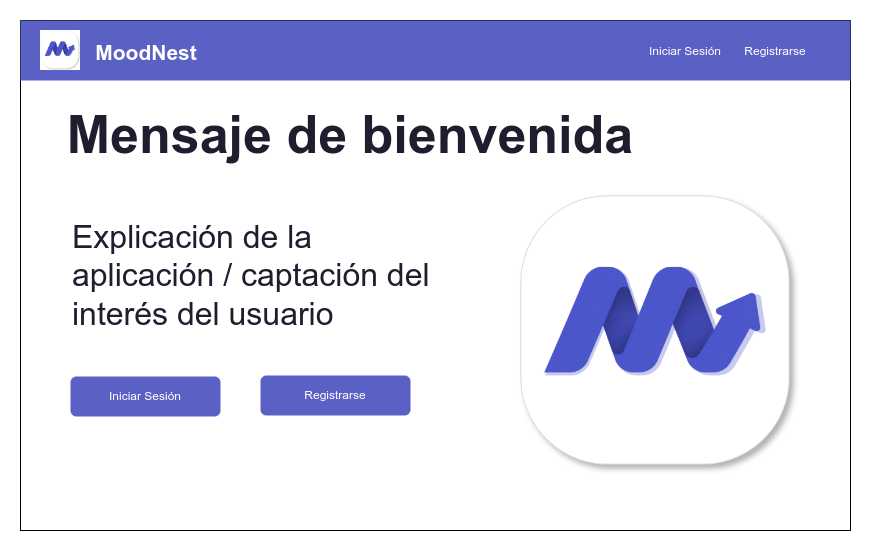
\includegraphics[width=\linewidth]{Imagenes/wf_bienvenida.png}
        \caption{Pantalla de Bienvenida y Onboarding.}
        \label{fig:wf_bienvenida}
    \end{minipage}\hfill
    \begin{minipage}{0.45\textwidth}
        \centering
        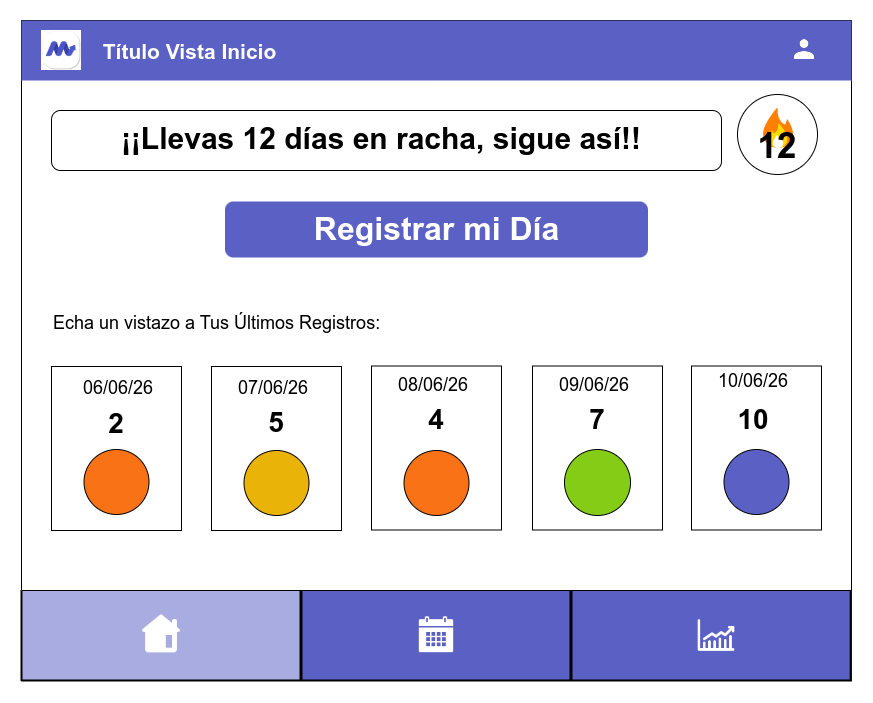
\includegraphics[width=\linewidth]{Imagenes/wf_inicio.png}
        \caption{Vista de Inicio (Dashboard con racha).}
        \label{fig:wf_inicio}
    \end{minipage}
\end{figure}

Como se observa en la Figura \ref{fig:wf_bienvenida}, el primer punto de contacto del usuario es una vista de bienvenida que explica el valor de la aplicación y capta su interés antes del acceso. Una vez dentro, la vista de Inicio (Figura \ref{fig:wf_inicio}) focaliza la atención en la retención del usuario mediante un mensaje motivacional basado en su racha de días consecutivos, ofreciendo además un acceso rápido a sus últimos registros históricos.

\begin{figure}[H]
    \centering
    \begin{minipage}{0.45\textwidth}
        \centering
        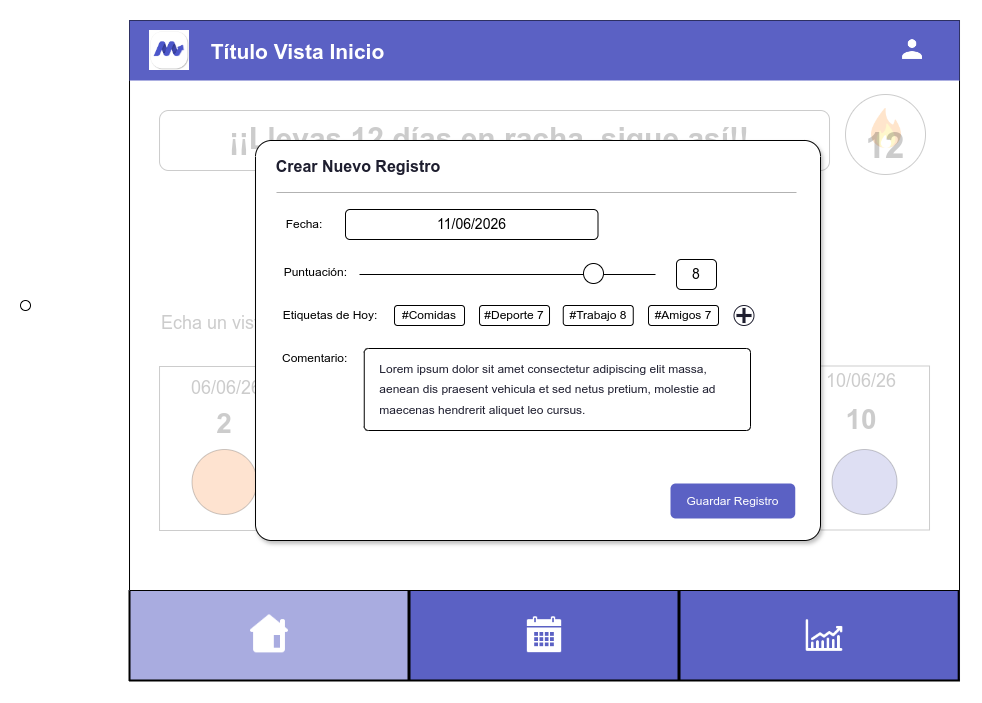
\includegraphics[width=\linewidth]{Imagenes/wf_registro.png}
        \caption{Formulario de Nuevo Registro.}
        \label{fig:wf_registro}
    \end{minipage}\hfill
    \begin{minipage}{0.45\textwidth}
        \centering
        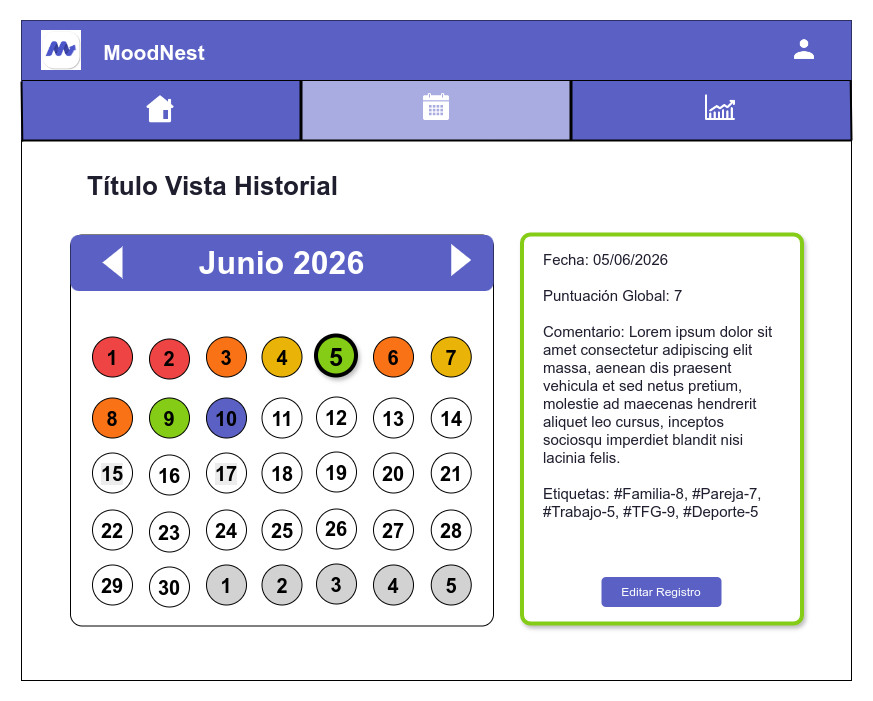
\includegraphics[width=\linewidth]{Imagenes/wf_historial.png}
        \caption{Vista Historial (Calendario mensual).}
        \label{fig:wf_historial}
    \end{minipage}
\end{figure}

El núcleo interactivo de MoodNest recae en la creación y consulta de datos. La Figura \ref{fig:wf_registro} muestra el formulario de creación de un nuevo registro diario, diseñado para que el usuario pueda crear un registro diario de la forma más rapida y simple posible. Por su parte, la Vista Historial (Figura \ref{fig:wf_historial}) actúa como un mapa de calor mensual donde cada día refleja la puntuación del usuario para ese día, permitiendo desplegar los detalles y etiquetas de un día concreto interactuando directamente sobre el calendario.

\begin{figure}[H]
    \centering
    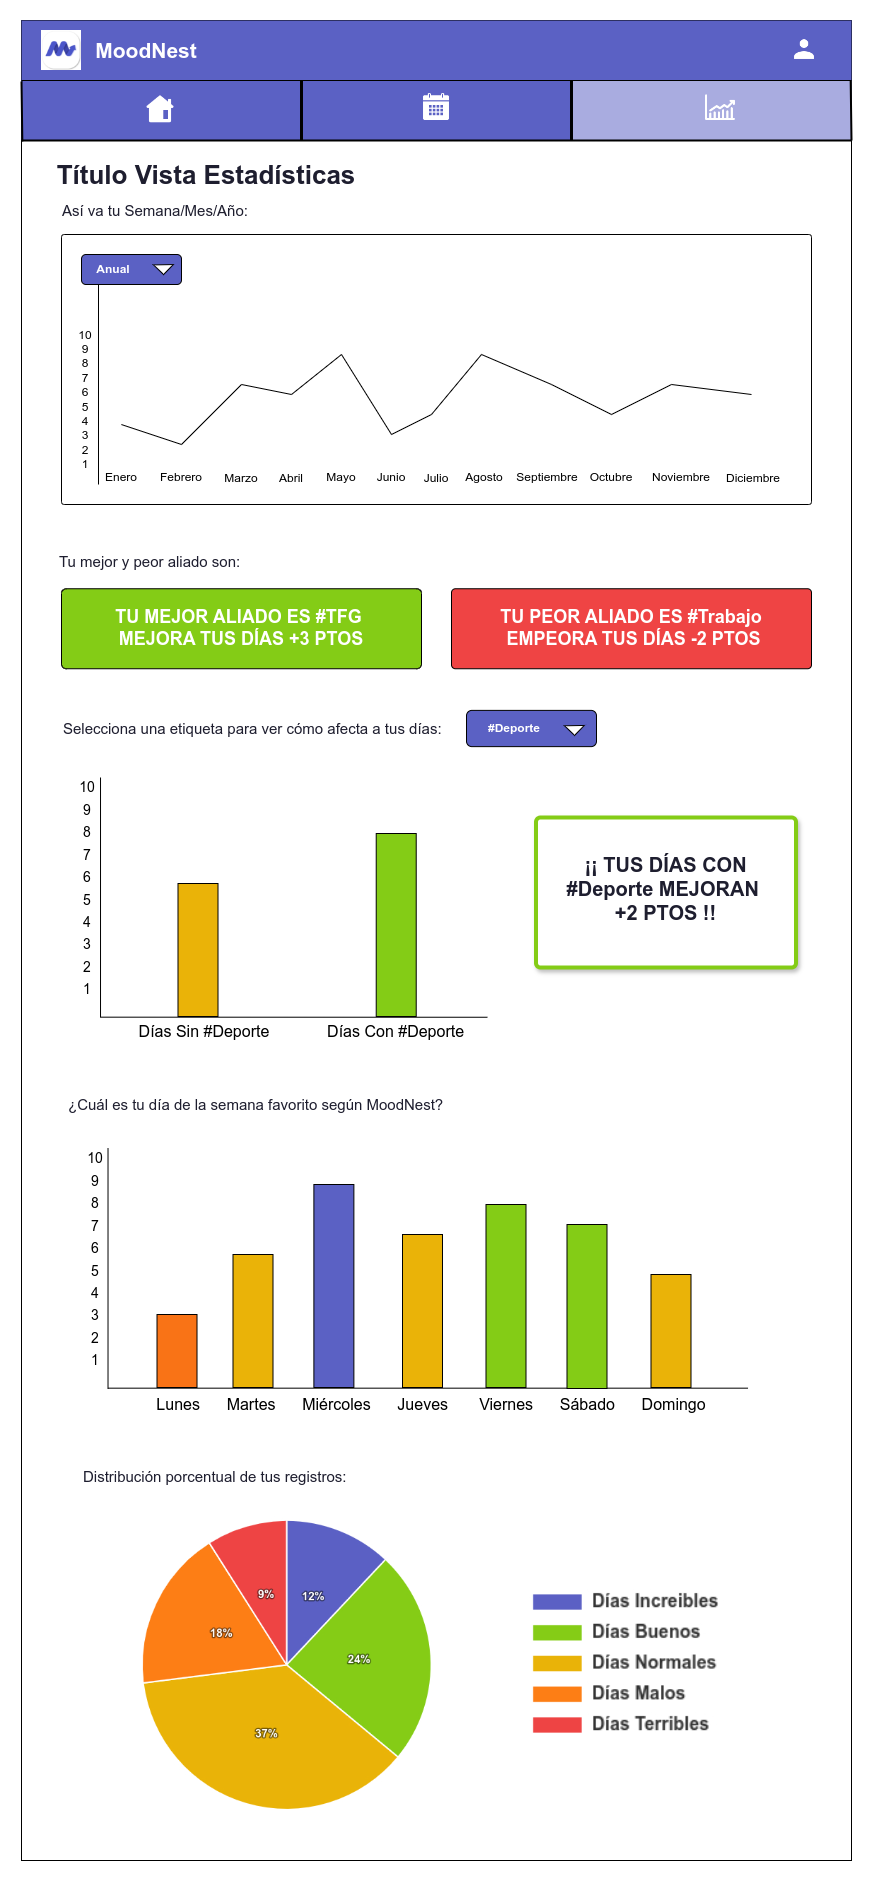
\includegraphics[width=0.45\textwidth]{Imagenes/wf_estadisticas.png}
    \caption{Vista de Análisis Estadístico.}
    \label{fig:wf_estadisticas}
\end{figure}

Finalmente, la Figura \ref{fig:wf_estadisticas} expone el panel analítico. Esta vista traduce los datos brutos en descubrimientos de valor, identificando mediante un análisis automatizado qué etiquetas actúan como el ''mejor o peor aliado'' del usuario, cuantificando su impacto directo en el estado de ánimo y presentando distribuciones porcentuales en gráficos circulares y de barras.